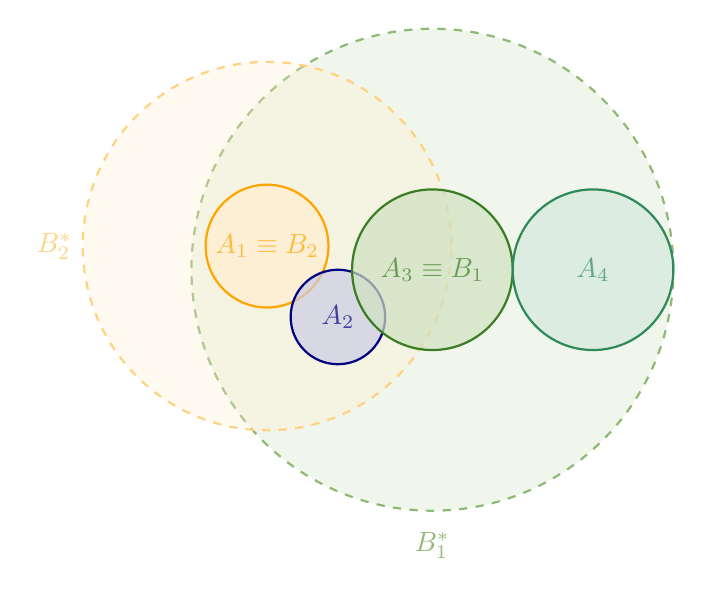
\begin{tikzpicture}[scale=0.6]
\draw[thick, dashed, OliveGreen!50!white, fill = OliveGreen!20!white, fill opacity = 0.3] (3.5, -0.5)  circle (5.1cm) node [yshift=-3.5cm, opacity=1] {$B_1^*$};
\draw[thick, dashed, Orange!50!white, fill = Orange!20!white, fill opacity = 0.3] (0,0) circle (3.9cm)  node [xshift=-2.7cm, opacity=1] {$B_2^*$};

\draw[thick, Orange, fill = Orange!20!white, fill opacity = 0.7] (0,0) node {$A_1 \equiv B_2$} circle (1.3cm);
\draw[thick, NavyBlue, fill = NavyBlue!20!white, fill opacity = 0.7] (1.5, -1.5) node {$A_2$} circle (1cm);
\draw[thick, OliveGreen, fill = OliveGreen!20!white, fill opacity = 0.7] (3.5, -0.5) node {$A_3 \equiv B_1$} circle (1.7cm);
\draw[thick, SeaGreen, fill = SeaGreen!20!white, fill opacity = 0.7] (6.9, -0.5) node {$A_4$} circle (1.7cm);

\end{tikzpicture}
